\section{biguint-mul}
\label{biguint-mul}

\begin{enumerate}
    \item target
        \begin{itemize}
            \item implement the multiplication of two biguints
        \end{itemize}
    \item constraints-logic
        \begin{itemize}
            \item compute mul-factors first, use U32ArithmeticGate
            \item add mul-factors from low bits, use U32AddManyGate
        \end{itemize}
    \item mul-process layout
        \begin{figure}[!ht]
            \centering
            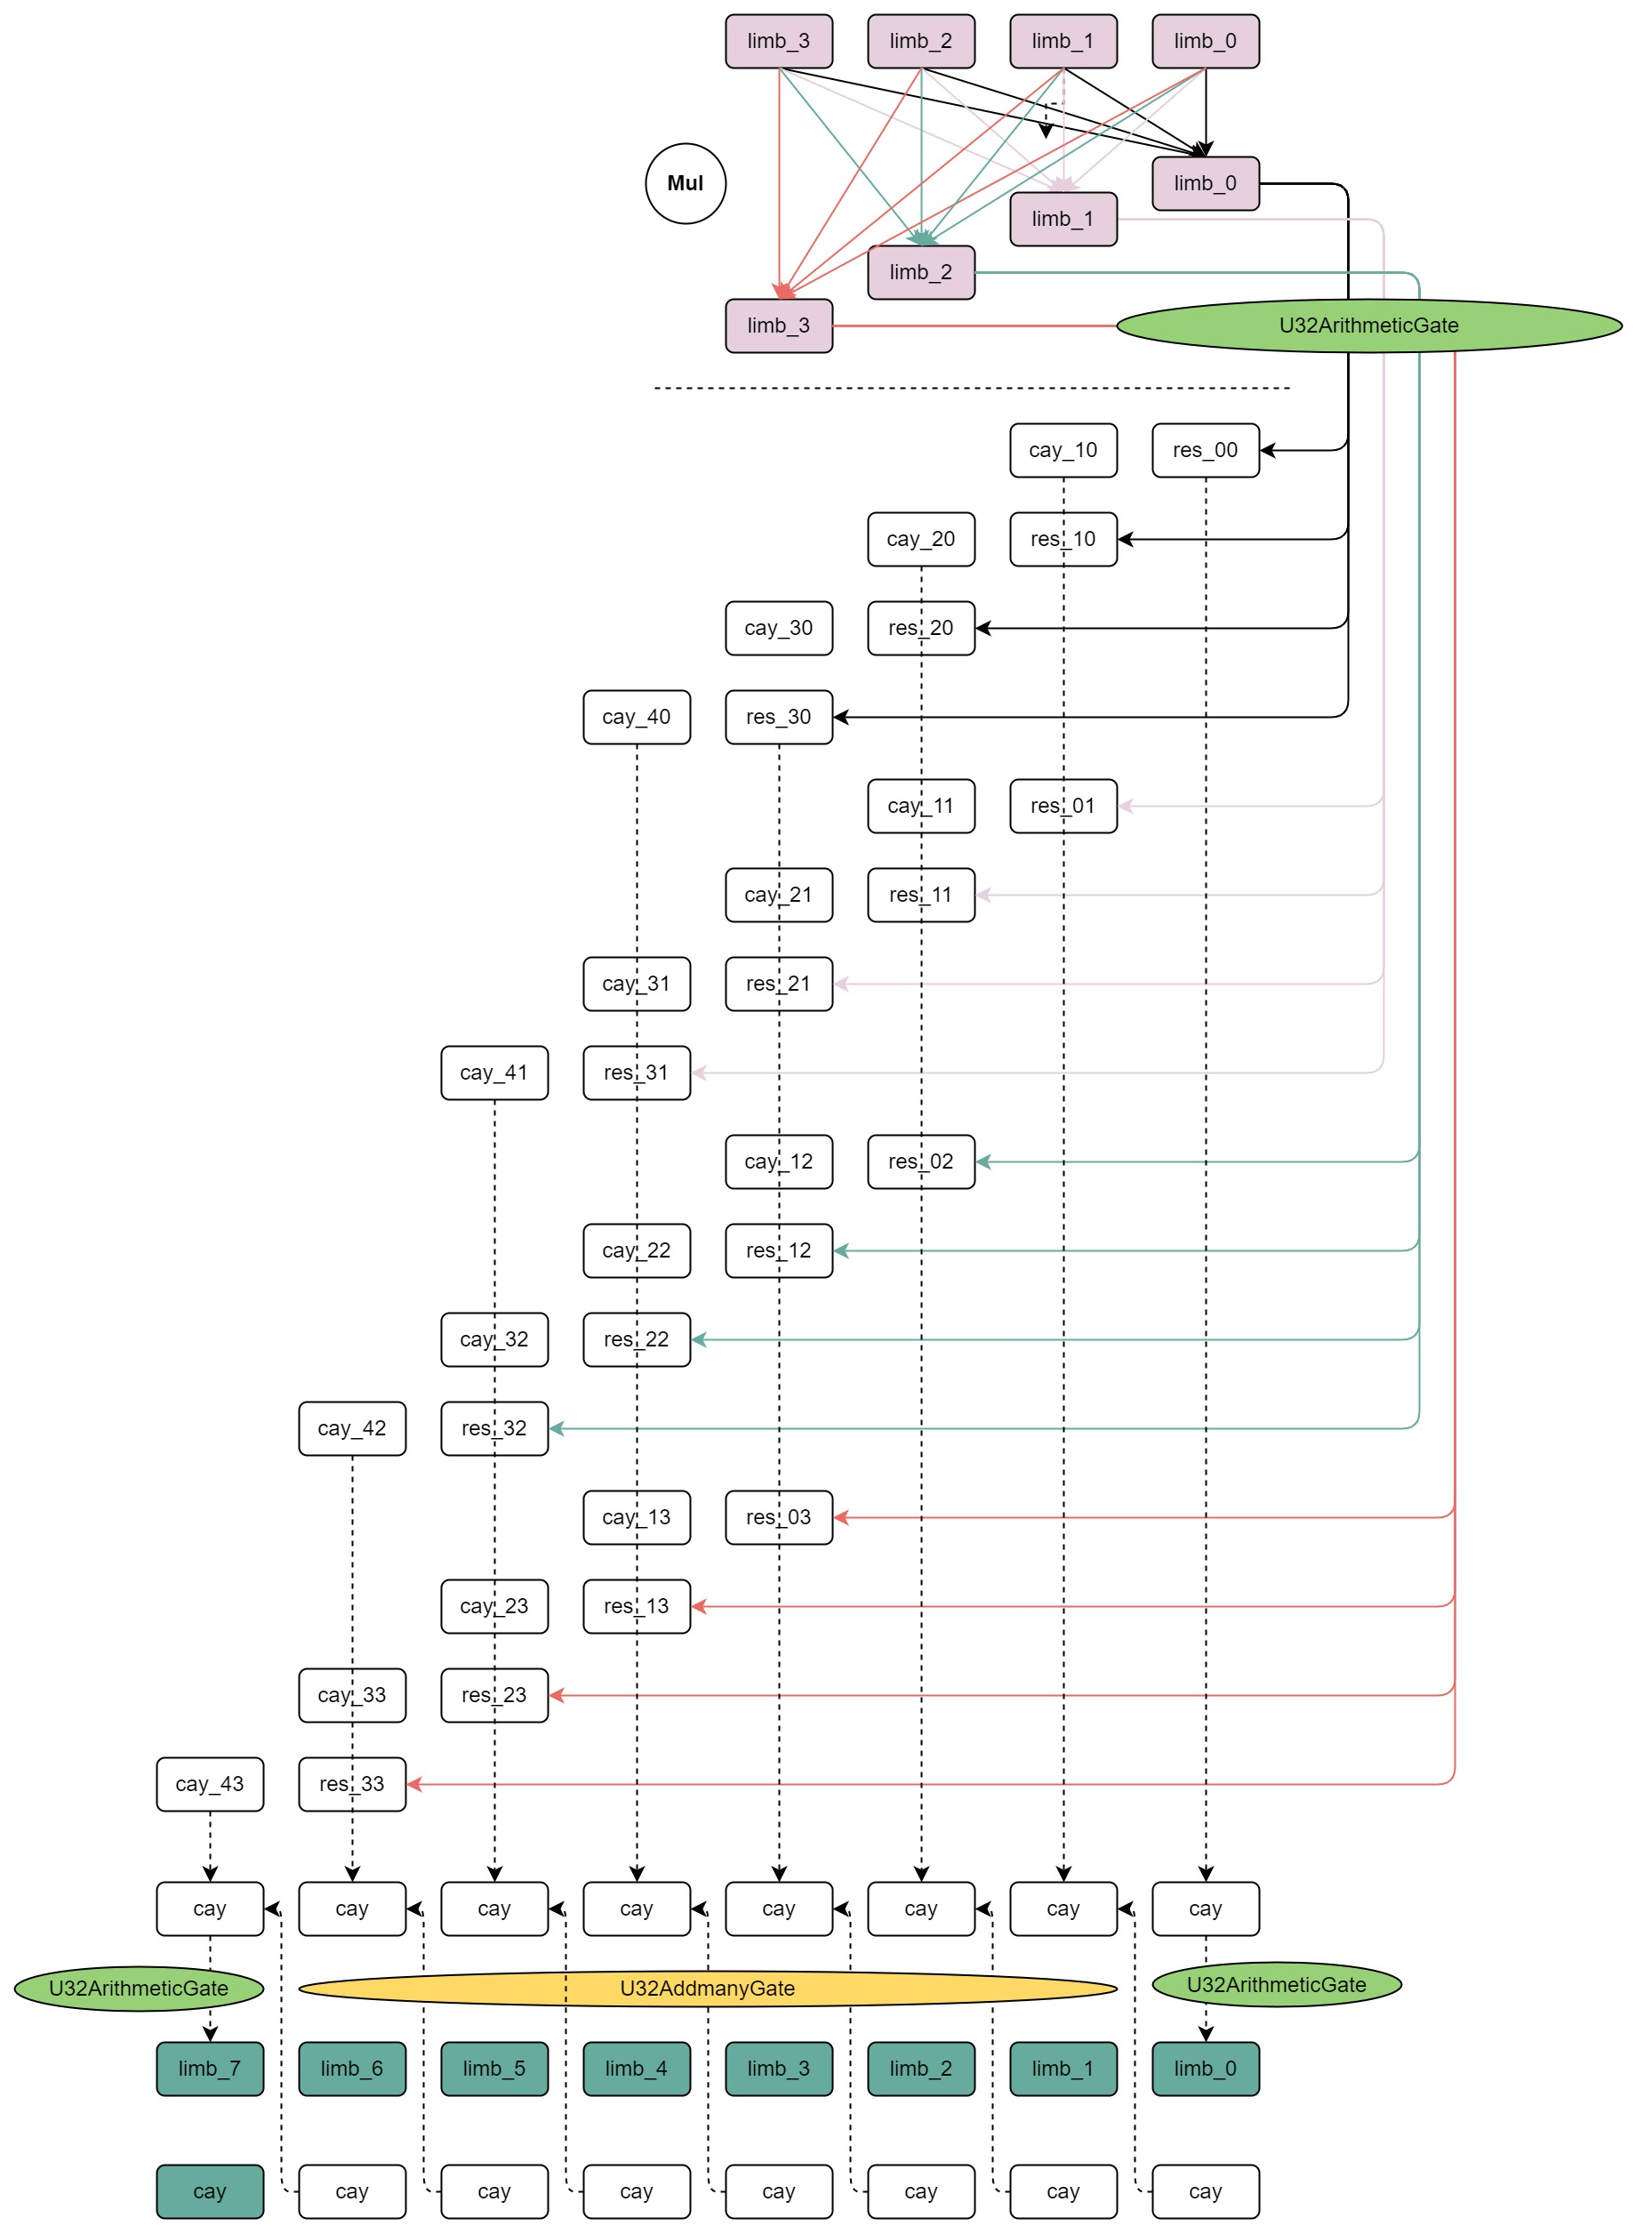
\includegraphics[width=0.8\textwidth]{biguint-mul-layout.jpg}
            \caption{biguint-mul layout.jpg}
            \label{fig:biguint-mul-layout.jpg}
        \end{figure}
    
    \item constraints-info and costs
        \begin{itemize}
            \item Gate type num: 4(U32ArithmeticGate, U32AddManyGate(num-addends: 4), U32AddManyGate(num-addends: 6), U32AddManyGate(num-addends: 8))
            \item Gate instance num: 9
            \item U32ArithmeticGate num: 6
            \item U32AddManyGate num: 3
            \item copy-constraints: 18 * 3 + (4 + 6 + 8) * 2 + 9 = 99
            \item max-degree: 4
        \end{itemize}

\end{enumerate}